\section{GRAFT}
\label{sec:method}

GRAFT is a deterministic post-training quantizer for weights released on an MXFP4 grid. It codes each matrix
$W\in\mathbb{R}^{k\times n}$ ($k$ inputs, $n$ outputs) at 3 bits per weight with a trellis whose decoded values are
MXFP4 blocks, combined with per-column scales (\cref{fig:pipeline}).

\begin{figure}[b!]
\centering
\begin{tikzpicture}[font=\scriptsize, node distance=2.2mm,
  box/.style={draw=black!55, rounded corners=1.5pt, fill=#1, minimum height=6mm, align=center, inner sep=2pt},
  box/.default=white, ar/.style={-{Stealth[length=1.5mm]}, black!60}]
\node[box=blue!6] (state) {16-bit\\state $s$};
\node[box, right=of state] (hash) {$h=$ bytesum\\$(s\cdot\texttt{0x83DCD12D})$};
\node[box=green!7, right=of hash] (map) {$2^{1-f}\,\mathrm{E2M1}\big(\tfrac{h-510}{w_f}\big)$};
\node[box=orange!8, below=3mm of map] (tail) {$|h-510|\le d$:\\$2^{-f}(\pm2^m\{1,1.5\})$};
\node[box, right=of map] (scale) {$\times\,2^{p_j}\alpha_j$};
\draw[ar] (state) -- (hash); \draw[ar] (hash) -- (map); \draw[ar] (map) -- (scale);
\draw[ar] (hash.south) |- (tail.west); \draw[ar] (tail.east) -| (scale.south);
\end{tikzpicture}
\caption{Decoding one weight. The state is the 16-bit window of the bitstream that ends at the current step, and the
hash is EXL3's. GRAFT's value map is the hardware E2M1 conversion, scaled by the flag $f\in\{0,1\}$ of the weight's
32-input block, or, for states at the hash centre, a power-of-two ladder (tail). No inverse rotation is needed.
Outside the tail every block is an MXFP4 block with scale $2^{1-f}$, and the tail values form an exact sparse
correction.}
\label{fig:pipeline}
\end{figure}

\paragraph{Trellis.} GRAFT uses EXL3's 16-bit bitshift trellis, which codes each 16$\times$16 tile in tensor-core
order as one tail-biting ring of 256 steps. At 3 bits per weight the decoder shifts in three bits per step, so a tile
holds 768 bits.

\paragraph{The grid-aligned codebook.} GRAFT keeps EXL3's hash $h(s)$ but replaces the value map. A weight in
row $i$ and column $j$ belongs to the MX block of rows $32\lfloor i/32\rfloor$ to $32\lfloor i/32\rfloor+31$ of
column $j$. If this block has flag $f\in\{0,1\}$ ($f=0$ in a matrix without flags), the weight's trellis state $s$
decodes to
\begin{equation*}
v(s)=2^{-f}\begin{cases}\pm 2^{m}\{1,1.5\} & |h-510|\le d,\\
2\,\mathrm{E2M1}\big(\tfrac{h-510}{w_f}\big) & \text{otherwise},\end{cases}
\end{equation*}
with $h=h(s)$. The bulk value is computed as $\mathrm{E2M1_{RNE}}(\mathrm{fp32}((2^{23}+h)q_a^{(f)}+q_b^{(f)}))$
with $q_a^{(f)}=1/w_f$ and $q_b^{(f)}=-(2^{23}+510)q_a^{(f)}$, which takes one fused multiply-add and the GPU's E2M1
conversion. In an unflagged block the bulk takes the 15 values $\{0,\pm1,\pm2,\pm3,\pm4,\pm6,\pm8,\pm12\}$, and a
flagged block decodes to half these values, $\{0,\pm0.5,\dots,\pm6\}$, with its own width $w_1$. A column normalized
by one power of two contains blocks whose MXFP4 scale is an octave below the column's, and the flag gives these blocks
the grid they need. The width $w_f$ sets how the Gaussian-like hash spreads over the grid. A tail state takes its sign
from bit 0 of $s$ and its magnitude from $\rho=(s\gg1)\bmod 26$ as $2^{3+\lfloor\rho/2\rfloor}$, multiplied by 1.5
if $\rho$ is odd, which gives 26 magnitudes from 8 to $49{,}152$ (\cref{fig:qtail}). Because the bulk map outputs
zero at the hash centre, the band trades a small part of the zero mass for range. It covers
\final{TAIL-D0} states (0.27\%) at $d=0$ and \final{TAIL-D20} (10.7\%) at $d=20$. The fit uses $d=0$ on
\final{BAND0} of the matrices and never more than $d=\final{BANDMAX}$, and \final{BAND-LATE} of the others lie in the
last three layers, where the outliers are.

\paragraph{Decoded representation.} Outside the tail, $v=2^{1-f}e$ with $e$ an E2M1 value, so every (32-input block,
column) pair of a GRAFT matrix decodes to an OCP MXFP4 block, that is, to E2M1 codes with the power-of-two block
scale $2^{1-f}$. The flag is the block's MX scale stored in one bit. The full reconstruction is
$\widehat W=(B+T)\,\mathrm{diag}(c)$, where $B$ holds these MXFP4 blocks, $T$ is the sparse tail and
$c_j=2^{p_j}m_g\alpha_j$ is the column scale. The matrix $B$ is MXFP4, but $\widehat W$ in general is not, because
$\alpha_j$ is a free fp16 factor and tail values lie outside their block's range. Both are applied outside the
block-scaled product. A tail value is an exact FP8 number, which a decoder applies as a sparse correction
next to the block at the cost of one product per tail weight (\final{TAILS} of the weights in our fits). Every decoded value is $0$ or $\pm2^e\{1,1.5\}$, an exact FP8 E5M2 number.

\begin{figure}[t]
\centering
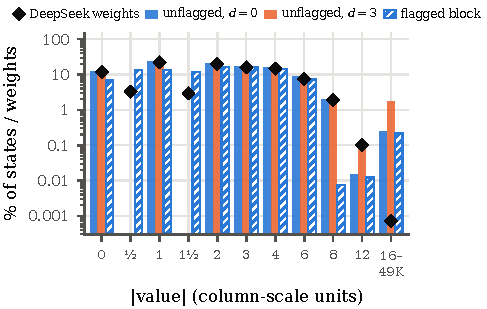
\includegraphics[width=\linewidth]{figures/fig_qtail}
\caption{GRAFT's codebook compared with its source. Bars: share of the 65,536 trellis states that decode to each
magnitude in an unflagged block (width 95.68) at tail band $d=0$ and $d=3$, and in a flagged block (hatched; its own
table at width 53, the most common width in the fit, halved). The last bar pools the tail ladder $2^m\{1,1.5\}$,
$m=3..15$, up to 49,152. Diamonds: share of DeepSeek-V4.1-Flash's routed-expert weights at each magnitude in the same
column units (\final{SRC-N} matrices). On the grid the codebook follows the source, including zero (\final{ZERO-D0}
of the states, \final{SRC-ZERO} of the weights). The halves (\final{SRC-HALF} of the weights) lie in blocks an octave
below their column's MX scale, and a flagged block's table puts \final{FLAGTAB-HALF} of its states on them. To reach
the outliers, which are rare (\final{SRC-TAIL} of these weights lie above 12), the tail takes its states from the hash
centre, where the bulk decodes to zero (\final{ZERO-D3} of the states at $d=3$). The fit uses $d=0$ on \final{BAND0}
of the matrices.}
\label{fig:qtail}
\end{figure}

\paragraph{Scales.} Each column is scaled by $2^{p_j}m_g\alpha_j$. The first factor is a power of two that brings to
3 the RMS of the column's weights that lie within $16\times$ its RMS, so that a few huge weights, which the tail codes,
do not inflate it. The second is a power-of-two multiplier $m_g\in\{1,2,4,8\}$ for densely heavy columns, shared by
each group of 16 columns (one tile wide). The third is an fp16 factor $\alpha_j$, computed in closed form after the fit
as the $H$-weighted least-squares fit of the decoded column. Free (non-power-of-two) scales give \final{FREE-SCALES}
more error.

\paragraph{Parameter selection.} The widths, the tail band $d$, the group multipliers and the flags are all chosen
with one quantity, the \emph{fit-weighted tile error}
\begin{equation*}
E=\sum_{t}\frac{1}{p_t}\sum_{(i,j)\in t} \delta_i s_j\,(\hat w_{ij}-w_{ij})^2 ,
\end{equation*}
which is the error of the trellis when it codes a $16\times16$ tile $t$ on its own (without error feedback) under the
per-weight costs of the fit ($\delta_i$ is the block-LDL diagonal of the shrunk $H$ and $s_j$ the column weight),
summed over 256 tiles drawn with probability $p_t$ proportional to their share of $\sum\delta_i s_j w_{ij}^2$. Without
flags, $(w_0,d)$ is chosen by coordinate descent, and each group's multiplier by the same error over all of the
group's tiles. At those scales we try three flag rules, each with its own widths. The first flags every block for
which rounding its scaled weights onto the halved grid gives the lower fit-weighted error, and the other two flag the
blocks whose largest scaled magnitude is at most 4 or at most 5. A rule with flags is charged a factor of $4^{1/32}$,
which is what its $1/32$ bit per weight is worth on the Gaussian rate curve, and the cheapest of the four options is
fitted. Sampling the tiles by importance under the fit's costs matters, because uniform, unweighted tiles misjudge
matrices whose error concentrates in a few heavy rows.

\paragraph{Objective and encoder.} For each matrix the fit minimizes $\sum_j s_j(w_j-\hat w_j)^\top H(w_j-\hat w_j)$
over its columns $w_j$. In the input-by-output convention, a gated MLP with gate pre-activations $z=W_1^\top x$ and
up activations $u=W_3^\top x$ computes $y=W_2^\top\big(\phi(W_1^\top x)\odot W_3^\top x\big)$ (with the model's
activation clamps). The squared sensitivity of the
expert output to gate channel $j$ at token $t$ is $\sigma^{(1)}_{tj}=(\phi'(z_{tj})u_{tj})^2\|W_2[j,:]\|^2$, and to up
channel $j$ it is $\sigma^{(3)}_{tj}=\phi(z_{tj})^2\|W_2[j,:]\|^2$. We approximate each by the product of a column
weight $s_j\propto\sum_t\sigma_{tj}$, normalized to mean 1, and a token weight $\omega_t=\sum_j\sigma_{tj}$, which
gives $H=\sum_t\omega_t x_tx_t^\top/\sum_t\omega_t$. For the down projection, $H$ comes from the quantized gate/up
activations and $s=1$. We shrink $H$ 25\% toward its diagonal and add 1\% damping. The encoder runs reverse
block-LDL error feedback with a weighted tail-biting Viterbi search over all $2^{16}$ states per 16-row block, in
which each position's flag selects its value table. The path cost weights each position by the block-LDL diagonal and
its column weight, $\delta_i s_j$.

\paragraph{MXFP4 operands.}
\label{sec:operands}
Because $B$ consists of MXFP4 blocks, its product runs on existing block-scaled tensor-core GEMMs. A block-scaled
FP4 or FP8 matrix multiply (W4A4, W4A8) takes the E2M1 codes and the block scales $2^{1-f}$ as they are and applies the
column scale per output channel in the epilogue, and the tail correction is a sparse product added to the result. A
W8A8 kernel sees the same values as exact FP8 numbers. The reference implementation of DeepSeek-V4.1-Flash quantizes
each expert activation to E4M3 with one power-of-two scale per 32 inputs and multiplies it with the MXFP4 weights in a
block-scaled FP4 GEMM. To run a GRAFT matrix on this path, a decoder first converts its trellis to MXFP4 codes and
block scales. The GEMM itself is unchanged, and its result receives the column scale (one FP32 multiply per output)
and the sparse tail product. With the native weights, the same path reproduces the reference bit for bit. In our
evaluation the conversion of each layer's experts happens before the GEMM. This validates numerical compatibility, but
decoding inside the GEMM, which keeps the weights compressed in memory, is not measured here.

\paragraph{Storage.} Each matrix stores the trellis words, a rate code, a codebook code, six fp32 constants
($q_a,q_b$ for each flag state and $d$), the fp16 column scales and, if the matrix uses flags, one bit per 32-input
block and column. This amounts to $3kn+16n+208$ bits, plus $kn/32$ with flags, which gives \final{BPW-NOFLAG} bits per
weight on DeepSeek's experts without flags and \final{X-BPW} on average with them (EXL3 at 3.0 stores
\final{BPW-EXL3}). The code consists of the trellis words alone, with no escapes or side tables.
